\documentclass[10pt,twocolumn]{article}

\usepackage[margin=0.72in]{geometry}
\usepackage[T1]{fontenc}
\usepackage[utf8]{inputenc}
\usepackage{times}
\usepackage{amsmath,amssymb}
\usepackage{graphicx}
\usepackage{booktabs}
\usepackage{caption}
\usepackage[hidelinks]{hyperref}
\usepackage{xcolor}
\usepackage{titlesec}

\captionsetup{font=small,labelfont=bf,skip=4pt}
\titlespacing*{\section}{0pt}{6pt}{3pt}
\titlespacing*{\subsection}{0pt}{5pt}{2pt}
\titleformat{\section}{\normalfont\large\bfseries}{\thesection}{0.6em}{}
\titleformat{\subsection}{\normalfont\normalsize\bfseries}{\thesubsection}{0.6em}{}
\setlength{\parskip}{0pt}
\setlength{\abovedisplayskip}{4pt}
\setlength{\belowdisplayskip}{4pt}

\newcommand{\lam}{\lambda}

\title{\vspace{-2.2em}\textbf{Adaptive Thinking for Tool Use:}\\[2pt]
\large Why a Length Penalty Cannot Teach a Small Model \emph{When} to Reason}

\author{Walid Ajbar\\[2pt]
\small MSc AI \& Data Management for Sustainability (AIDAMS), ESSEC / CentraleSup\'elec\\
\small \texttt{walidajbar05@gmail.com} \quad Code: \url{https://github.com/widodu77/rs_aidams}}
\date{\vspace{-0.6em}\small August 2026}

\begin{document}
\maketitle

\begin{abstract}
\noindent
Reasoning models emit a chain of thought before every action, including actions
that need none. We ask whether a 1.7B model can be trained, with GRPO and a
reward of the form \emph{correctness $-\ \lam\cdot$ think tokens}, to reason only
on the tool calls that warrant it. It cannot, and the reason is structural rather
than a matter of tuning. We report three findings. (i) The prize is real: a
per-item oracle over two fixed policies is both more accurate and $2.7\times$
cheaper than always reasoning, yet no prompt we tried collects any of it.
(ii) Across twelve trained runs the think rate never leaves $96$--$99\%$, because
GRPO standardises advantages within a group and on a group of equal correctness
the reward spread is \emph{itself} proportional to $\lam$, so $\lam$ divides out
of the update exactly. We verify the cancellation numerically on $344$ logged
steps. (iii) Relocating the decision from the prompt into the completion makes
$\lam$ reach the gradient, but a sweep across a fortyfold range of $\lam$ then
yields five behaviourally identical policies, all at $0\%$ think rate: the
objective has no interior optimum for any $\lam>0$. What survives is a clean
statement about tool use at this scale. Reasoning before a function call is
\emph{purchasable}: it costs roughly $200$ tokens per call and buys no measurable
accuracy ($89.9\%$ versus $89.5\%$, McNemar $p{=}1.000$, $-204.5$ tokens/item).
\end{abstract}

\section{Introduction}

A reasoning model asked for today's weather in Paris will often deliberate for
two hundred tokens before emitting a one-line function call. The deliberation is
not free, and on a call this easy it is not obviously useful. The natural
objective is a \emph{gate}: reason on the calls where reasoning pays, answer
directly on the rest. Recent work trains length-controlled reasoners with
reinforcement learning by adding a length term to the reward
\cite{arora2025efficient,aggarwal2025l1}, and the overthinking literature
documents the waste such a gate would recover \cite{chen2024overthinking}. The
obvious recipe is therefore GRPO \cite{shao2024deepseekmath} on
\[
  r = w_c\,\mathbf{1}[\text{correct}] + w_f\,\mathbf{1}[\text{well formed}]
      - \lam \cdot \frac{\min(t,B)}{B},
\]
with $t$ the number of thinking tokens and $B$ a budget, and then a sweep over
$\lam$ to trace a cost--quality frontier.

We ran that recipe carefully, on a benchmark whose official checker we reuse as
the reward, and it does not work. This paper reports why, because the reason
generalises past our setup: it is a property of the interaction between a
$\text{correct}-\lam\cdot\text{length}$ reward and GRPO's group normaliser, not
a property of our model, our task, or our hyperparameters.

\textbf{Contributions.} \emph{(1)} We establish that the target is worth wanting
and that prompting cannot reach it (\S\ref{sec:prize}). \emph{(2)} We show that
$\lam$ cancels exactly out of the normalised advantage whenever a GRPO group
agrees on correctness, derive the identity, and confirm it to $<10^{-5}$ on
$344$ logged training steps (\S\ref{sec:cancel}). \emph{(3)} We repair the
rollout so that $\lam$ does reach the gradient, and show that the resulting
objective has a cliff rather than a curve: five values of $\lam$ spanning $40\times$
give five indistinguishable policies (\S\ref{sec:cliff}). The by-product is a
measurement worth reporting on its own, namely that chain of thought before a
function call is purchasable at this scale (\S\ref{sec:purchasable}).

\section{Setup}

\textbf{Task and scoring.} We use the single-turn portion of the Berkeley
Function Calling Leaderboard \cite{bfcl,patil2023gorilla}: $1240$ items across
\texttt{simple\_python} ($400$), \texttt{multiple} ($200$), \texttt{parallel}
($200$), \texttt{parallel\_multiple} ($200$) and \texttt{irrelevance} ($240$).
Correctness is BFCL's own abstract-syntax-tree checker, wrapped as a per-sample
scorer so that the training reward and the reported accuracy are the same
function. Numbers therefore stay comparable to the public leaderboard. The split
is $992$ train / $248$ held out, fixed by a seeded manifest; every number below
is on the held-out $248$ unless stated.

\textbf{Model and training.} Qwen3-1.7B \cite{qwen3}, chosen because it can
reason and call a function in a single turn and exposes an explicit
thinking-mode switch. GRPO via TRL \cite{trl} with LoRA \cite{hu2021lora}
($r{=}32$, $\alpha{=}64$), $100$ optimiser steps, $8$ generations per group,
learning rate $10^{-5}$, completions capped at $B{=}768$ tokens, seed $0$. The
reward uses $w_c{=}1.0$, $w_f{=}0.2$, and $\lam \in \{0.05, 0.25, 0.5, 1.0, 2.0\}$.
Because the length term is normalised by $B$, $\lam$ reads directly as the
maximum price of a reasoning block in units of correctness.

\textbf{A precision caveat that changed our conclusions.} Our first baselines
were 4-bit NF4, forced by a 4\,GB local card. At fp16 two of those findings
reversed sign. Quantisation had damaged the \emph{never-reason} policy
specifically (\texttt{parallel} accuracy $18\%\rightarrow69\%$), so what looked
like a benefit of reasoning was reasoning masking quantisation damage. All
numbers in this paper are fp16.

\section{Finding 1: the prize is real, and no prompt collects it}
\label{sec:prize}

Table~\ref{tab:anchors} gives three fixed policies and a per-item oracle that
picks, for each item, the cheaper of the two that gets it right.

\begin{table}[t]
\centering\small
\begin{tabular}{lrrr}
\toprule
policy & acc. & tokens & think rate\\
\midrule
never reason        & 71.4\% & 51.4 & 0\%\\
always reason       & 89.5\% & 264.1 & 98.4\%\\
``reason only if needed'' & 89.1\% & 280.6 & 96.8\%\\
\midrule
per-item oracle     & \textbf{92.7\%} & \textbf{99.5} & 17.4\%\\
\bottomrule
\end{tabular}
\caption{Held-out $248$ items. The oracle is simultaneously more accurate than
always reasoning and $2.7\times$ cheaper, so a gate is worth $3.2$ accuracy
points \emph{and} $165$ tokens per call. The adaptive prompt collects none of it.}
\label{tab:anchors}
\end{table}

The oracle reasons on $17.4\%$ of items. That number is the target, and it is
also the collapse diagnostic used throughout: a policy at $0\%$ or at $98\%$ is
not gating, whatever its accuracy.

Asking for the behaviour does not produce it. Three separate prompt wordings,
including one that lists the direct answer format first and states that most
calls do not need reasoning, all leave the think rate above $96\%$; the adaptive
prompt is the most expensive policy in the table and no more accurate than
always reasoning. The model does not lack the capacity to answer directly, since
the never-reason policy demonstrates it. It lacks any pressure to choose.

\section{Finding 2: $\lam$ cancels out of the GRPO update}
\label{sec:cancel}

We trained ten adapters, two sweeps of five $\lam$, differing in whether each
group was free-sampled or forced to contain both thinking modes, plus two
further runs varying the advantage normaliser. All twelve land between $87.9\%$
and $90.7\%$ accuracy at $224$--$281$ tokens with think rates of $96.4$--$99.6\%$.
No pairwise McNemar test among them reaches $p<0.05$. The frontier does not move,
in any direction, for any $\lam$.

The cause is exact and can be written down. GRPO standardises the reward within
each group of $G$ rollouts,
\[
  A_i = \frac{r_i - \operatorname{mean}(r)}{\operatorname{std}(r) + \varepsilon},
  \qquad \varepsilon = 10^{-4}.
\]
Suppose every rollout in the group receives the same correctness and format
verdict, so $r_i = K - \lam\, t_i / B$ with $K$ constant. Then
\[
  r_i - \operatorname{mean}(r) = -\tfrac{\lam}{B}\big(t_i - \bar t\,\big),
  \qquad
  \operatorname{std}(r) = \tfrac{\lam}{B}\operatorname{std}(t),
\]
and therefore
\[
  A_i \;=\; \frac{-\big(t_i - \bar t\,\big)}{\operatorname{std}(t) + \varepsilon B/\lam}
  \;\xrightarrow[\ \varepsilon \to 0\ ]{}\;
  \frac{-\big(t_i - \bar t\,\big)}{\operatorname{std}(t)} .
\]
The advantage is a $z$-score of \emph{length alone}, and $\lam$ has vanished from
it. Doubling the price of thinking does not double the gradient; it changes
nothing except through the stabiliser $\varepsilon$, whose residual effect we
measure as an attenuation factor
$\operatorname{std}(r)/(\operatorname{std}(r)+\varepsilon)$ of $0.982$ to $0.999$
across our runs. This is the entire purchase $\lam$ makes.

The condition is not a corner case. Instrumenting all $500$ logged training steps
of the five paired runs, correctness and format are constant across the group on
$344$ of them ($68.8\%$), and on those steps the identity above holds to a maximum
relative error of $9.7\times10^{-6}$. On the remaining $31\%$, correctness varies
and $\lam$ can genuinely reorder rollouts, but that is too thin a channel to move
a policy in $100$ steps.

The observation that GRPO's standard-deviation division distorts the objective
has been made before, on different grounds and with a different remedy
\cite{liu2025drgrpo}. Our point is sharper and specific to length-penalised
rewards: the normaliser does not merely bias the update, it removes the
experimental variable. Any study that sweeps $\lam$ in a
$\text{correct}-\lam\cdot\text{length}$ reward under vanilla GRPO is, on most of
its steps, running the same experiment repeatedly.

\textbf{A second, avoidable error.} Our paired runs forced half of each group to
answer directly by prefilling the empty thinking block into the \emph{prompt}.
This makes the direct branch off-policy: its reinforcement lands on a prompt that
is never used at evaluation. It also removes all within-branch length pressure.
Pairing consequently made reasoning \emph{longer} than free sampling ($+32.9$
tokens/item, $95\%$ CI $[+23.1, +43.0]$), the opposite of its intent.

\begin{figure}[t]
\centering
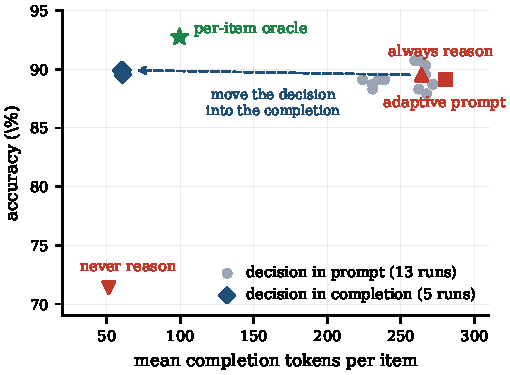
\includegraphics[width=\columnwidth]{figures/frontier.pdf}
\caption{Cost against quality on the held-out $248$. Thirteen runs whose thinking
decision sat in the prompt (grey: the twelve of \S\ref{sec:cancel} plus the
control of \S\ref{sec:cliff}) are indistinguishable from always reasoning at
every $\lam$. Moving the decision into the completion (blue) collapses cost by
$77\%$ at the same accuracy, but overshoots the oracle to $0\%$ think rate.}
\label{fig:frontier}
\end{figure}

\section{Finding 3: repairing the rollout exposes a cliff}
\label{sec:cliff}

The diagnosis names its own fix. If the decision is made in the prompt, the
completion begins \emph{after} the choice and the choice is never in the space
the policy is optimised over. So we moved it. Our \emph{gate rollout} keeps one
prompt for the whole group and forces the direct half by prepending the empty
thinking marker to its \emph{completion}. The marker is derived at run time by
diffing the two chat-template renderings rather than hardcoded. Both branches are
now on-policy, pairing is legitimate, and at evaluation the model emits the
decision itself.

It works, in the mechanical sense. Think rate moves for the first time in the
project: from $0.45$, the forced fraction, to $0.00$ (Figure~\ref{fig:collapse}).
The control differs in exactly one respect and does not move at all.

Then we swept $\lam$ over the same fortyfold range. Table~\ref{tab:sweep} is the
result. All five runs are the same policy. The endpoints, trained under a
fortyfold difference in the price of a thinking token, disagree on \emph{one}
held-out item out of $248$ ($p{=}1.000$; $+1.4$ tokens, $[+0.3,+2.8]$). They are
not duplicate checkpoints: pairwise, $91$--$93\%$ of their raw completions are
byte-identical rather than $100\%$, so $\lam$ moves the weights. It moves nothing
observable.

\begin{table}[t]
\centering\small
\begin{tabular}{lrrr}
\toprule
$\lam$ & acc. & tokens & think rate\\
\midrule
0.05 & 89.5\% & 61.0 & 0\%\\
0.25 & 89.5\% & 60.7 & 0\%\\
0.5  & 89.9\% & 60.9 & 0\%\\
1.0  & 89.5\% & 60.7 & 0\%\\
2.0  & 89.9\% & 59.7 & 0\%\\
\bottomrule
\end{tabular}
\caption{The $\lam$ sweep with the decision in the completion. A $40\times$ range
in the price of thinking produces one policy.}
\label{tab:sweep}
\end{table}

\textbf{Why a cliff and not a curve.} This is the same cancellation one level up.
On a group of equal correctness the only reward variance is length, so the
standardised advantage is $\pm1$ regardless of $\lam$: $\lam$ selects the
\emph{sign} and nothing else. The sign points toward shorter completions in every
group where reasoning fails to flip a correctness verdict, which at 1.7B on
single-turn tool calls is nearly every group. Hence
\[
  \arg\min_{\text{think rate}} \; \mathbb{E}\,[\text{correct}] - \lam \cdot \text{length}
  \;=\; 0 \quad \text{for all } \lam > 0,
\]
unless correctness depends on length, and our fixed-policy table already says it
barely does. There is no interior optimum, so no value of $\lam$ finds one, and
every run walks to the boundary within $27$ steps and then freezes: once all eight
rollouts agree, $\operatorname{std}(r)=0$ and the remaining seventy-odd steps are
no-ops. The first cancellation removed $\lam$ from the magnitude of the update.
The second removes $\lam$ from the answer.

\begin{figure}[t]
\centering
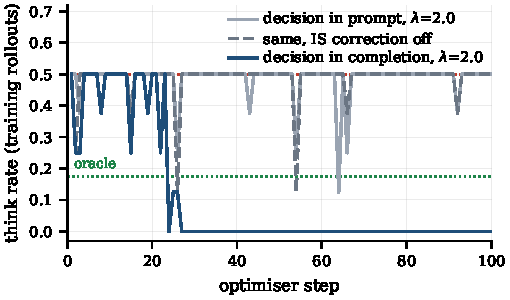
\includegraphics[width=\columnwidth]{figures/collapse.pdf}
\caption{Think rate over \emph{training rollouts} at $\lam{=}2.0$. Half of every
group is forced to answer directly, so $0.5$ is a floor imposed by the rollout,
not a learned rate: the two prompt-decision runs never leave it in $100$ steps,
and at evaluation both still reason on $98\%$ of items. Moving the decision into
the completion makes $\lam$ act, and the policy walks straight past the oracle's
$17.4\%$ to zero by step $23$.}
\label{fig:collapse}
\end{figure}

\section{What survives: reasoning is purchasable}
\label{sec:purchasable}

The $0\%$ policy is not degenerate, and comparing it against the anchors gives
the one result here that a practitioner can use directly
(Table~\ref{tab:sig}). It matches always-reasoning on accuracy at $4.4\times$
lower cost, and beats the cost-matched never-reason prompt on $46$ items while
losing zero.

\begin{table}[t]
\centering\small
\setlength{\tabcolsep}{4pt}
\begin{tabular}{lccr}
\toprule
gate ($\lam{=}2.0$) vs. & win/loss & $p$ & $\Delta$tokens [95\% CI]\\
\midrule
always reason      & 13 / 12 & 1.000 & $-204.5$ $[-220,-190]$\\
decision in prompt & 12 / 11 & 1.000 & $-207.2$ $[-222,-194]$\\
adaptive prompt    & 13 / 11 & 0.839 & $-221.0$ $[-238,-205]$\\
never reason       & 46 / \phantom{0}0 & $<$0.001 & $+8.3$ $[+5.7,+11.3]$\\
\bottomrule
\end{tabular}
\caption{Paired tests on the same $248$ items. Accuracy by exact McNemar
\cite{mcnemar1947}; token differences by paired bootstrap, $10^4$ resamples.
Win/loss counts only the items the two policies disagree on.}
\label{tab:sig}
\end{table}

Every completion is a real call. Per category against never-reason:
\texttt{parallel} $72.5\rightarrow92.5$, \texttt{parallel\_multiple}
$50.0\rightarrow72.5$, \texttt{irrelevance} $37.5\rightarrow93.8$, with correct
multi-call output and correct prose abstention. So on single-turn BFCL at 1.7B,
\textbf{chain of thought before a function call costs about $200$ tokens and buys
nothing measurable.} Deployments that reason by default on tool calls at this
scale are paying for it.

\textbf{Two caveats we hold to.} First, this is not the gate: $0\%$ is not
$17.4\%$, and the model did not learn \emph{when} to reason, it learned not to
need reasoning. Second, the comparison against never-reason confounds training
with gating, since never-reason is prompted and this is trained. The honest
control is the other twelve trained runs, identical in reward and budget, which
saved no tokens at all ($224$--$281$ versus $59.7$). That contrast is what
attributes the saving to the rollout design rather than to training in general.

\section{Limitations}

One task family, one model, one seed per configuration, $100$ optimiser steps,
and LoRA rather than full fine-tuning. The winning run collapsed and then froze,
so roughly three quarters of its steps did nothing. Our hypothesis that thinking
would concentrate on harder categories was never testable, because think rate sat
at $90$--$100\%$ in every category of every policy: there was no variance to
correlate difficulty against. Finally, the $\arg\min$ argument in
\S\ref{sec:cliff} is a statement about our reward and our accuracy--length
relationship, not a theorem about all tool-use tasks; on a domain where reasoning
genuinely flips correctness often, the interior optimum would exist.

\section{What a gate would actually need}

The failure is informative because it is specific. A gate requires a reward whose
\emph{sign} varies within a group, which $\text{correct}-\lam\cdot\text{length}$
does not provide once accuracy is length-insensitive. Three routes follow, none
tested here: price errors asymmetrically so that reasoning pays on the hard
slice; impose a per-category or per-item token budget so the comparison is
between allocations rather than between lengths; or add an entropy floor on the
gate decision to stop the collapse at step $23$ and keep both branches alive long
enough to be compared. We would also expect the effect to be larger on
multi-turn or multi-step tool use, where an early mistake compounds and reasoning
has something to buy.

\section{Related work}

Chain-of-thought prompting made intermediate reasoning a default rather than a
choice \cite{wei2022cot}, and RL with verifiable rewards made it a trained
behaviour \cite{guo2025deepseekr1}; a recent survey catalogues the resulting
design space \cite{zhang2025survey}. The cost of that default is now well
documented: o1-style models spend many tokens on trivial problems
\cite{chen2024overthinking}. Two lines of work respond. One adds a length term to
the RL reward so the model learns to be shorter \cite{arora2025efficient}; the
other conditions on a requested budget so length becomes controllable at
inference \cite{aggarwal2025l1}. Both target the \emph{length} of reasoning on
problems that need some. We asked the adjacent question, whether the model can
learn to skip reasoning entirely on the calls that need none, and our result is
that the first approach cannot answer it under vanilla GRPO for a reason that is
not about tuning. The closest prior observation is the critique of GRPO's
standard-deviation normaliser as a source of bias \cite{liu2025drgrpo}; we show
that for a length-penalised reward the same normaliser does something stronger,
removing the swept variable rather than skewing it. Our setting also differs from
most of this literature in domain: it is tool use scored by an executable
checker \cite{bfcl,patil2023gorilla} rather than mathematics, and at 1.7B rather
than frontier scale, which is precisely the regime where our accuracy--length
relationship is flat enough to make the cliff appear.

\section{Reproducibility and use of LLMs}

Code, the seeded split manifest, all raw generations, and a dated research log
recording every failure in sequence are at
\url{https://github.com/widodu77/rs_aidams}. Every table here is regenerated from
raw generations by a single command; $116$ unit tests cover the scorer, the
reward, the rollout functions and the statistics.

An LLM assistant (Claude, Anthropic) was used for implementation and for drafting
this document. It wrote first versions of the analysis modules
(\texttt{lambda\_purchase.py}, \texttt{significance.py}, \texttt{pareto.py}), the
rollout functions, and the notebook plumbing. All statistical choices (exact
McNemar over $\chi^2$ because the discordant counts are under $20$; paired
bootstrap over a $t$-interval because token counts are heavily skewed) were
reviewed line by line, and the derivation in \S\ref{sec:cancel} was checked
against the logged training data before being believed. One prediction generated
during the work, that batch-level normalisation would amplify $\lam$'s effect,
was mine and was wrong; the controlled run showed the opposite, and it is
recorded as such in the research log.

\bibliographystyle{plain}
\bibliography{refs}

\end{document}
